\documentclass[10pt,letterpaper]{article}
\usepackage[T1]{fontenc}
\usepackage[utf8]{inputenc}
\usepackage{lmodern}
\usepackage[margin=0.90in]{geometry}
\usepackage{microtype}
\usepackage{amsmath,amssymb,mathtools}
\usepackage{graphicx}
\usepackage{booktabs,tabularx,array}
\usepackage{enumitem}
\usepackage[font=small,labelfont=bf]{caption}
\usepackage{float}
\usepackage{hyperref}
\hypersetup{
  colorlinks=true,
  linkcolor=black,
  citecolor=black,
  urlcolor=blue,
  pdftitle={From Shared Weights to Dark Fibers: Virtual Depth, Head-Readable Staircases, and Unmonitored Search in Looped Transformers},
  pdfauthor={Patrick Dugan}
}
\setlength{\parindent}{1.1em}
\setlength{\parskip}{0.18em}
\setlist[itemize]{topsep=3pt,itemsep=1.5pt,leftmargin=*}
\renewcommand{\arraystretch}{1.14}

\newcommand{\LoopT}{\textsc{Loop-T}}
\newcommand{\FFU}{\textsc{FF-U}}
\newcommand{\EM}{\ensuremath{\mathrm{EM}}}
\newcommand{\IIA}{\ensuremath{\mathrm{IIA}}}
\newcommand{\DEF}{\ensuremath{\mathrm{DEF}}}
\newcommand{\cur}{\operatorname{cur\_node}}
\newcommand{\Gprop}{G_{\mathrm{prop}}}
\newcommand{\Phead}{P_{\mathrm{head}}}

\title{\bfseries From Shared Weights to Dark Fibers:\\[0.32em]
Virtual Depth, Head-Readable Staircases, and\\[0.14em]
Unmonitored Search in Looped Transformers}
\author{Patrick Dugan}
\date{November 2026\\[0.2em]\normalsize Unified synthesis across \texttt{VPD}, \texttt{HUG-CAL-02}, \texttt{RMP}, \texttt{LOOPSCOPE-01}, and \texttt{LOOPSCOPE-02}}

\begin{document}
\maketitle
\vspace{-0.65em}

\begin{abstract}
\noindent
Weight-tied transformers reuse identical parameters across sequential passes, yet parameter sharing conflates distinct computational regimes whose capability gains, failure modes, and latent-state monitorability differ sharply. Synthesizing four experimental programs across pretrained looped language models (\texttt{Nanbeige4.2-3B}, \texttt{Huginn-0125}), controlled algorithmic loopers (\LoopT, \texttt{LoopedChase}, \texttt{Lean-CGRT}), untied baselines (\FFU, \texttt{Qwen3.5-4B-Base}, \texttt{Qwen3-4B-Instruct}), and 7M-parameter convergent Tiny Recursive Models (\texttt{TRM}), we separate weight sharing into three mechanistic regimes. First, two-pass language models implement \emph{fixed-pass virtual depth}: \texttt{Nanbeige4.2-3B} routes through layer-selectively distinct singular subspaces across passes ($\bar{r}=0.355$; $r=0.085$ at layer 12) and shifts downstream perturbation geometry when loop-boundary states are carried rather than reset, while top-$k$ sparse autoencoder support switching limits intervention-change fidelity ($F_\Delta > 0$ in 1 of 12 second-pass layer-22 conditions despite Muon raising state explained variance from $-0.180$ to $0.453$). Across pointer chasing, algebraic group composition (\texttt{ARG-02}), and deductively stratified $9\times 9$ Sudoku (\texttt{LOOPSCOPE-02}), two-pass reuse yields no out-of-distribution loop scaling and trails untied 4B baselines ($0.129$ vs.\ $0.211$, McNemar $p=0.0031$). Second, multi-iteration BPTT loopers exhibit \emph{dynamical settling and head-readable staircases}: matched input-read rotations on \texttt{Huginn-0125} (\texttt{HUG-CAL-02}) eliminate apparent late-iteration SVD factor specialization ($\pm 0.0065$ nats across 8 frozen factors), motivating \emph{Transported Component Attribution} (\texttt{TCA}), which separates dynamical fragility from closed-form directional specificity in one backward pass ($\rho=0.75$ across 480 ablations) and exposes a Lyapunov dichotomy between BPTT and 1-step detached ACT ($F_1/F_6 = 1{,}808.4$ despite $0.303\times$ finite kick contraction, alongside $22.04\%$ read-specific components). On Markovian pointer chains, intermediate supervision ($\lambda \ge 0.1$) yields $1.00$ depth-9--16 extrapolation and $1.00$ head readability with zero capability trade-off, while own-head belief commutation predicts extrapolation at $\mathrm{AUC}=0.992$. Third, on $9\times 9$ Sudoku, a 7M \texttt{TRM} solves $88.3\%$ of stratified boards and $100\%$ of \texttt{bench100} ($51/51$ deductively stalled boards): its visible beliefs commute with exact constraint propagation before stall ($\mathrm{AUC}=1.000$), yet erasing the 501-dimensional \texttt{lm\_head} nullspace of $z_H$ while preserving step-$s$ digit logits collapses exact solve from $1.000$ to $0.070$ ($p=2.02\times 10^{-28}$). Head-level monitoring suffices for Markovian propagation; non-monotone constraint search requires unmonitored dark-fiber state.
\end{abstract}

\section{Introduction: Three Regimes of Weight Sharing}\label{sec:intro}

A weight-tied transformer applies the same block parameters $\theta$ across $T$ sequential passes \cite{dehghani2019universal,giannou2023looped,saunshi2025latent,geiping2025huginn,jolicoeur2025trm}. Because parameter identity no longer indexes computational depth, two questions govern both capability and interpretability in recurrent-depth models:
\begin{enumerate}[topsep=3pt,itemsep=2pt]
  \item \textbf{Capability triangulation:} When does reusing $\theta$ across passes buy genuine multi-step algorithmic or combinatorial reasoning beyond an untied feedforward transformer, and what dynamical invariants separate non-extrapolating fixed-pass models from convergent recursive solvers?
  \item \textbf{Latent monitorability:} When can the intermediate trajectory of a looped computation be audited directly through its output readout head or a shared sparse dictionary, and when is task success causally carried by unmonitored subspaces orthogonal to the readout?
\end{enumerate}

Our September 2026 study of the pretrained two-pass language model \texttt{Nanbeige4.2-3B} \cite{dugan2026vpd} approached parameter reuse from the bottom up: decomposing shared MLP matrices via multipass vector parameter decomposition (\texttt{VPD}) \cite{braun2025apd} and fitting shared Top-$k$ sparse autoencoders (\texttt{SAE}s) \cite{bricken2023monosemanticity,gao2024scaling} across \texttt{ARC-AGI-1}, \texttt{ARC-AGI-2}, and \texttt{INTELLECT-3} reasoning traces. That investigation uncovered severe terminal-layer pass divergence, demonstrated that optimizer geometry (Muon vs.\ AdamW \cite{jordan2024muon}) rescues held-out second-pass state reconstruction without rescuing intervention-change fidelity, and proved via a 44-layer embedding-reset control that carrying loop-boundary state changes the physical response direction of downstream layers. Yet it left three structural questions open: whether two-pass reuse confers multi-step capability over untied models, whether per-pass or per-iteration ablation asymmetries reflect specialized weight factors or dynamical sensitivity, and whether deeper recurrent loops preserve head-accessible intermediate variables or hide state in unmonitored channels.

Over the subsequent ten weeks, five concurrent looped-transformer interpretability papers established important pieces of recurrent mechanics while leaving this capability--monitorability synthesis unresolved (Table~\ref{tab:literature}). Wu, Hu, and Zhang \cite{wu2026shared} showed via Jacobian steering that shared weights route inputs to distinct effective linear maps across passes; Sesodia et al.\ \cite{sesodia2026inside} documented iteration-budget difficulty staircases on depth-bound tasks; Blayney et al.\ \cite{blayney2026mechanistic} analyzed fixed-point convergence and feedforward stage emulation; Olszowiec et al.\ \cite{olszowiec2026monitoring} studied hidden-state stability and noise sensitivity during latent reasoning; and Kaissis et al.\ \cite{kaissis2026sdi} introduced Step-Decomposed Influence (\texttt{SDI}) using per-iteration activation--gradient outer products. However, none of these works (i) controlled per-step component attribution against closed-form orthogonal input/output rotations, (ii) tested open-loop and donor-displacement counterfactuals across fixed-pass language models and convergent Tiny Recursive Models (\texttt{TRM}s) on a shared deductively stratified NP-complete benchmark, or (iii) isolated the causal subspace separating head-readable propagation from non-monotone search.

\begin{table}[t]
\centering
\small
\begin{tabularx}{\linewidth}{@{}l>{\raggedright\arraybackslash}p{0.31\linewidth}>{\raggedright\arraybackslash}X@{}}
\toprule
Concurrent study & Principal contribution & Unresolved gap addressed in this synthesis \\
\midrule
Blayney et al.\ \cite{blayney2026mechanistic} & Fixed-point convergence and feedforward stage emulation in looped LMs & Contrasts non-convergent 2-pass LMs (\texttt{Nanbeige-3B}) against contractive 336-pass \texttt{TRM}s on identical Sudoku strata \\
Kaissis et al.\ (\texttt{SDI}) \cite{kaissis2026sdi} & Per-step gradient--activation outer products $\sum \delta_t \otimes a_t$ for data influence & Shows detached-ACT Jacobians inflate step-1 norms by $6{,}400\times$; \texttt{TCA} cancels $\|A_s\|$ via exact rotation nulls \\
Wu et al.\ \cite{wu2026shared} & Jacobian steering shows cross-loop routing to distinct linear operators & Shows cross-pass SVD multiplexing in \texttt{Nanbeige} ($\bar{r}=0.355$) yields zero multi-step gain over untied \texttt{Qwen-4B} \\
Sesodia et al.\ \cite{sesodia2026inside} & Iteration-budget staircases on depth-bound algorithmic benchmarks & Proves visible beliefs commute with exact $\Gprop$ ($\mathrm{AUC}=1.000$) before stall and require a 501-d dark fiber past stall \\
Olszowiec et al.\ \cite{olszowiec2026monitoring} & Stability regimes and hidden-state trajectories in looped LMs & Establishes the exact monitorability regime boundary via \texttt{lm\_head} row-space projection ($1.000 \to 0.070$) \\
\bottomrule
\end{tabularx}
\caption{Positioning relative to concurrent 2026 looped-transformer interpretability studies.}
\label{tab:literature}
\end{table}

This paper unifies our September \texttt{Nanbeige} manuscript \cite{dugan2026vpd} with three subsequent programs—registered \texttt{Huginn-0125} calibration (\path{HUG-CAL-02} \cite{dugan2026hugcal}), controlled closed-loop mediation and extrapolation laws (\texttt{RMP} \cite{dugan2026rmp}, \path{LOOPSCOPE-01}, and \path{ARG-02} \cite{dugan2026arg02}), and stratified $9\times 9$ Sudoku triangulation (\path{LOOPSCOPE-02})—to establish that weight-tied transformers populate three mechanistically distinct regimes:
\begin{itemize}
  \item \textbf{Regime I — Fixed-Pass Virtual Depth (Section~\ref{sec:regime1}):} Fixed $T=2$ language models (\texttt{Nanbeige4.2-3B}) use state carry to select pass-dependent linear subspaces across shared weights, acting as an untied $2L$-layer pipeline with compressed parameters. They neither contract toward task-conditioned attractors nor outperform untied 4B models on multi-step propagation, and top-$k$ encoder support switching breaks sparse linear edit accounting at the loop boundary.
  \item \textbf{Regime II — Dynamical Settling and Head-Readable Staircases (Sections~\ref{sec:fragility}--\ref{sec:regime2}):} Multi-iteration BPTT loopers (\texttt{Huginn-0125}, \LoopT, \texttt{LoopedChase}, \texttt{Lean-CGRT}) reuse a shared basis across visits. Apparent late-iteration SVD specialization on \texttt{Huginn-0125} vanishes under activation-matched input rotations (\texttt{HUG-CAL-02}); \texttt{TCA} formalizes this decomposition analytically. When the underlying task is a deterministic Markovian chain, loopers admit closed-loop sparse dictionaries, causal feature-level variable transfer, and exact own-head commutation ($\mathrm{AUC}=0.992$) with \emph{zero} trade-off between extrapolation capability and readout monitorability.
  \item \textbf{Regime III — Stationary Attractor Search with Dark-Fiber Memory (Section~\ref{sec:regime3}):} A 7M-parameter Attention-\texttt{TRM} unrolled across 16 outer ACT steps (336 layer passes) iterates a highly stationary outer operator ($\bar{r}_{\mathrm{outer}}=0.992$) that contracts finite perturbations ($0.303\times$) and repairs 10-cell board corruptions ($0.000 \to 0.887$). Prior to deductive stall, its visible beliefs form a head-readable $\Gprop$ staircase; past stall, solving NP-hard boards via conflict traversal and non-monotone cell flips depends causally on a \textbf{501-dimensional dark fiber} in the nullspace of \texttt{lm\_head} ($1.000 \to 0.070$ when erased).
\end{itemize}

\paragraph{Provenance and registration discipline.} Across all four programs, pre-registered decision rules and post-hoc mechanistic follow-ups are kept strictly distinct. Where a pre-registered composite rule returned \texttt{Not supported} or \texttt{Weak}—notably \texttt{HUG-CAL-02} factor specialization, \texttt{ARG-02} \texttt{H2a}, and \texttt{LOOPSCOPE-02} \texttt{P1}, \texttt{P2}, \texttt{P3}, and \texttt{P4}—we report the exact registered verdict verbatim alongside the structural phenomenon isolated by its sub-metrics. Earlier sealed manuscripts (\texttt{VPD} versions 1--8 and \texttt{papers/rmp\_looped\_mechinterp}) remain unmodified.

\section{Regime I: Two-Pass Virtual Depth, Support Switching, and Non-Extrapolation}\label{sec:regime1}

We begin with \texttt{Nanbeige/Nanbeige4.2-3B} (revision \texttt{451ed48c}), a pretrained decoder that executes 22 shared transformer layers twice per forward pass with a loop-boundary \texttt{RMSNorm} before language-model readout. Combining our September \texttt{VPD}/\texttt{SAE} study \cite{dugan2026vpd} with three downstream capability evaluations—3-shot pointer chasing (\texttt{Silico Stage 1}), 168-case algebraic group composition (\texttt{ARG-02} \cite{dugan2026arg02}), and 256-board deductively stratified $9\times 9$ Sudoku (\texttt{LOOPSCOPE-02})—clarifies both what two-pass parameter sharing changes internally and what it fails to buy externally.

\subsection{Terminal Pass Divergence and the Muon SAE Fidelity Gap}

In \cite{dugan2026vpd}, a 64-component multipass \texttt{VPD} decomposition (\texttt{prime-20260906T204058Z-561}, capturing $\approx 2.2\%$ of squared weight norm at \texttt{mlp.down\_proj} of physical layers 12 and 22) and shared 6,144-latent Top-32 \texttt{SAE}s were evaluated across 18 reasoning trajectories (8 calibration, 10 held-out across 8 task groups) spanning \texttt{ARC-AGI-1}, \texttt{ARC-AGI-2}, and \texttt{INTELLECT-3} logic and mathematics. Comparing Pass-1 and Pass-2 residual states at identical token positions revealed a sharp depth asymmetry: cross-pass cosine similarity stays tightly aligned at physical mid-layer \texttt{L12} ($0.799$--$0.869$ across the four task families) but plunges at terminal physical layer \texttt{L22} to $0.230$--$0.307$ ($0.184$--$0.229$ after the loop-boundary \texttt{RMSNorm}). Crucially, this terminal divergence is already established inside the prompt suffix prior to autoregressive generation, indicating an architectural pass-routing split rather than chain-of-thought drift.

Training a single Top-32 dictionary across both passes initially failed on \texttt{L22} Pass 2 under AdamW, yielding negative held-out state explained variance ($\mathrm{EV} = -0.180$ on Q4 trajectories and $-0.535$ on BF16 intervention baselines, vs.\ $+0.830$ and $+0.763$ on Pass 1). Replacing AdamW with a Muon-hybrid optimizer \cite{jordan2024muon} under identical architecture and token budgets rescued static state reconstruction, lifting \texttt{L22} Pass-2 $\mathrm{EV}$ to $+0.453$ (Q4) and $+0.312$ (BF16) while raising Pass-1 $\mathrm{EV}$ to $0.918$ and $0.942$.

Static reconstruction, however, did not imply causal intervention fidelity. For a parameter-space write producing true residual shift $\Delta h = h_1 - h_0$ and dictionary-reconstructed shift $\Delta \hat{h} = \hat{h}_1 - \hat{h}_0$, write the exact identity $\Delta h = \Delta \hat{h} + (e(h_1) - e(h_0))$ with reconstruction error $e(h) = h - \hat{h}$, and define intervention-change fidelity
\begin{equation}
  F_\Delta \;=\; 1 - \frac{\|\Delta h - \Delta \hat{h}\|_2^2}{\|\Delta h\|_2^2}
  \;=\; 1 - \frac{\|e(h_1) - e(h_0)\|_2^2}{\|\Delta h\|_2^2}.
  \label{eq:fdelta}
\end{equation}
Although Muon improved \texttt{L22} Pass-2 $F_\Delta$ in $12/12$ tested intervention conditions ($18/20$ nonzero \texttt{L22} conditions overall), \emph{only $1/12$ crossed zero} (\texttt{L12} both-pass $+0.05$ scale: $F_\Delta = +0.030$, cosine $0.412$). Token-resolved error decomposition localized the failure mechanism: discrete Top-32 encoder support switches at just $1$--$3$ of $80$ sequence positions accounted for $93.3\%$--$99.6\%$ of total change-mismatch energy on local \texttt{L22} Pass-2 edits. Freezing the encoder's active support on a unit negative write collapsed $F_\Delta$ mismatch from $-52.367$ to $-0.000543$.

To separate loop-boundary state carry from executing 44 physical layers, \cite{dugan2026vpd} introduced a 44-layer \emph{embedding-reset control} that replaces the Pass-1 output with clean token embeddings at the loop boundary. Across 150 prompt--position pairs, reset Pass-2 states matched 22-layer one-pass states bit-for-bit ($0.0$ state and logit error). Under matched-norm residual writes ($\alpha \in \{0.1, 1, 10\}$) at \texttt{L12}, propagated \texttt{L12}$\to$\texttt{L22} Muon $F_\Delta$ remained positive under reset ($+0.047$ to $+0.572$) and negative under carry ($-0.300$ to $-0.046$). Crossing baseline states ($h_0^{\mathrm{carry}}$ vs.\ $h_0^{\mathrm{reset}}$) offline against unit perturbation directions proved that state carry rotates the \emph{downstream Jacobian response direction} ($\text{Muon } F_\Delta = 0.059/0.051$ for the carry response direction vs.\ $0.354/0.377$ for the reset direction regardless of baseline anchor).

\subsection{Triangulating Capability Across Pointer Chasing, Algebra, and Stratified Sudoku}

Does this state-carried cross-pass subspace routing buy multi-step reasoning capability over an untied transformer? Three independent evaluations answer in the negative (Figure~\ref{fig:triangulation}, Table~\ref{tab:sudoku_triangulation}):

\begin{figure}[t]
\centering
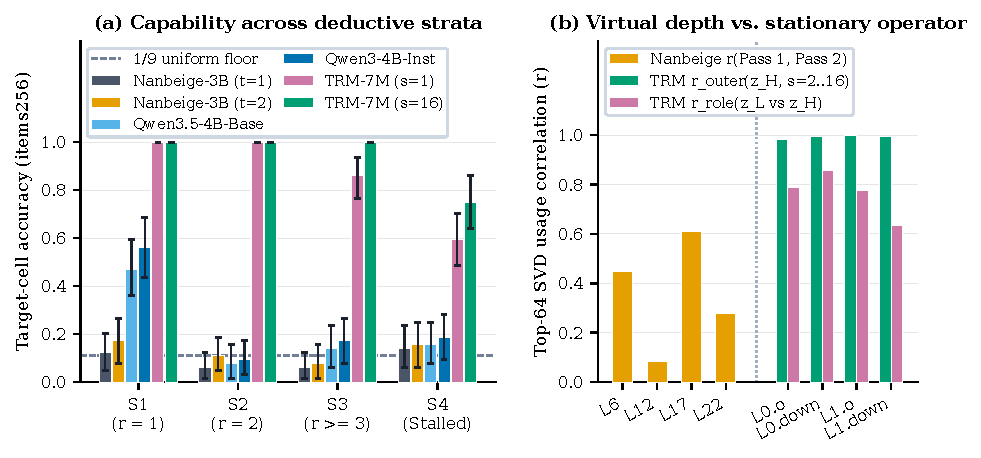
\includegraphics[width=\linewidth]{figures/fig1_virtual_depth_triangulation.pdf}
\caption{\textbf{Regime I vs.\ Regime III on deductively stratified $9\times 9$ Sudoku (\texttt{LOOPSCOPE-02}).} \textbf{(a)} Target-cell accuracy across 256 distinct boards ($n=64$ per stratum; error bars show 2,000-resample paired bootstrap 95\% CIs). Both \texttt{Nanbeige4.2-3B} ($t=1,2$) and untied 4B \texttt{Qwen} models collapse near the $1/9$ floor once deduction requires $r\ge 2$ rounds (\texttt{S2--S4}), whereas a 7M \texttt{TRM} achieves $1.000$ on \texttt{S1--S3} and $0.750$ single-cell ($0.836$--$1.000$ full-board) on stalled \texttt{S4}. \textbf{(b)} Top-64 SVD input-activation correlations: \texttt{Nanbeige} multiplexes layer-selectively across passes ($\bar{r}=0.355$), whereas \texttt{TRM} iterates a stationary outer operator ($\bar{r}_{\mathrm{outer}}=0.992$) while splitting inner $z_L$ vs.\ $z_H$ roles ($\bar{r}_{\mathrm{role}}=0.765$).}
\label{fig:triangulation}
\end{figure}

\begin{enumerate}[topsep=3pt,itemsep=2pt]
  \item \textbf{Multi-hop pointer chasing (\texttt{Silico Stage 1}):} On 3-shot 16-node pointer chasing (\path{exp_01m6dqy2dtehvtp4932aaqy9gy}), \texttt{Nanbeige4.2-3B} reaches $79.2\%$ at 1 hop (chance $6.25\%$) and collapses to $6.55\%$ ($131/2{,}000$) across depths 3--6. On a 120-item 1-hop \texttt{VPD} ablation sweep over the 64 Paper-I factors, \texttt{L12} matches random directions while three \texttt{L22} factors \texttt{(19, 9, 43)} cost $-0.060$ to $-0.098$ nats exclusively on Pass 1 ($0.000$ on Pass 2), with cross-pass usage correlation $r = 0.05$ (\texttt{L12}) and $0.06$ (\texttt{L22}).
  \item \textbf{Algebraic group composition (\texttt{ARG-02} Extension N1 \cite{dugan2026arg02}):} Evaluated across $t \in \{1, 2, 4, 8\}$ passes on 168 deterministic finite-group program traces (\texttt{future@12}), \texttt{Nanbeige4.2-3B} scores $44 / 65 / 76 / 71$—roughly matching single-pass untied \texttt{Qwen3.5-0.8B} ($68$) and trailing single-pass \texttt{Qwen3.5-2B} ($79$) and exact search ($159$). Registered recurrent mechanism gate \texttt{H2a} was not met: linear open-loop extrapolation $h_{\mathrm{open}}(t) = h(1) + (t-1)(h(1)-x)$ already recovers $55$ at $t=2$ ($+11$ via logit norm sharpening; $55$ vs.\ $71$ at $t=8$, McNemar $p=0.097$), donor-shuffled Pass-2 displacements score $69$ vs.\ $65$ clean (differing on $6/168$ cases), relative step norms remain $0.63$--$1.28$ without fixed-point convergence, and $0.25\cdot\mathrm{RMS}$ perturbations \emph{amplify} by $2.8\times \to 3.9\times \to 6.9\times$ at loops $2, 4, 8$.
  \item \textbf{Deductively stratified $9\times 9$ Sudoku (\texttt{LOOPSCOPE-02}):} Using an exact synchronous naked- plus hidden-single propagation operator $\Gprop$ over all 27 Sudoku units, we sampled 256 distinct held-out boards from \texttt{sudoku-extreme-1k}, stratified equally ($n=64$) into immediate 8-clue elimination (\texttt{S1\_naked1}, $r=1$), two-round propagation (\texttt{S2\_prop2}, $r=2$), deep propagation (\texttt{S3\_prop3plus}, $r\ge 3$), and strict round-0 zero-single boards requiring search (\texttt{S4\_stalled}). Under identical 3-shot single-token prompting, \texttt{Nanbeige4.2-3B} moves from $0.098$ ($t=1$) to $0.129$ ($t=2$, $+0.031$, McNemar $p=0.341$) and degrades at out-of-distribution loop counts ($0.090$ at $t=8$, $p=0.220$). Untied \texttt{Qwen3.5-4B-Base} ($0.211$, $p=0.0031$) and pure-SDPA \texttt{Qwen3-4B-Instruct-2507} ($0.254$) substantially outperform \texttt{Nanbeige} on immediate elimination (\texttt{S1}: $0.469$ and $0.562$ vs.\ $0.172$), while \emph{all three} 3B--4B language models collapse onto the $1/9 \approx 0.111$ uniform floor on multi-step strata \texttt{S2--S4} ($0.115$ vs.\ $0.125$, $p=0.824$). Top-64 SVD input-activation profiles $|(X v_r)|\sigma_r$ across physical layers \texttt{(6, 12, 17, 22)} confirm layer-selective multiplexing ($\bar{r}_{\mathrm{pass1,pass2}} = 0.355$: near-orthogonal at \texttt{L12} $r=0.085$ and \texttt{L22} $r=0.277$; moderately shared at \texttt{L6} $r=0.448$ and \texttt{L17} $r=0.610$).
\end{enumerate}

\begin{table}[t]
\centering
\small
\begin{tabularx}{\linewidth}{@{}lcccccc>{\raggedright\arraybackslash}X@{}}
\toprule
Model / Pass setting & Params & Overall & \texttt{S1} ($r{=}1$) & \texttt{S2} ($r{=}2$) & \texttt{S3} ($r{\ge}3$) & \texttt{S4} (Stall) & Loop / operator signature \\
\midrule
\texttt{Nanbeige4.2-3B} ($t=1$) & 3.0B & 0.098 & 0.125 & 0.062 & 0.062 & 0.141 & Half virtual pipeline (22 layers) \\
\texttt{Nanbeige4.2-3B} ($t=2$, native) & 3.0B & 0.129 & 0.172 & 0.109 & 0.078 & 0.156 & Multiplexed SVD ($\bar{r}=0.355$) \\
\texttt{Nanbeige4.2-3B} ($t=8$, OOD) & 3.0B & 0.090 & 0.047 & 0.156 & 0.062 & 0.094 & Non-contractive ($\|\Delta h\|/\|h\|=0.71$) \\
\texttt{Qwen3.5-4B-Base} (untied) & 4.0B & 0.211 & 0.469 & 0.078 & 0.141 & 0.156 & Untied 36L; mid-lens \texttt{L18} $= 0.109$ \\
\texttt{Qwen3-4B-Instruct} (SDPA) & 4.0B & 0.254 & 0.562 & 0.094 & 0.172 & 0.188 & Untied 36L pure-SDPA control \\
\midrule
\texttt{TRM-7M} ($s=1$: 18 passes) & 7.0M & 0.863 & 1.000 & 1.000 & 0.859 & 0.594 & Inner propagation; exact board $= 0.082$ \\
\texttt{TRM-7M} ($s=16$: 336 passes) & 7.0M & \textbf{0.938} & \textbf{1.000} & \textbf{1.000} & \textbf{1.000} & \textbf{0.750} & Stationary ($\bar{r}=0.992$); board $= \mathbf{0.883}$ \\
\bottomrule
\end{tabularx}
\caption{Stratified $9\times 9$ Sudoku target-cell accuracy on \texttt{items256} ($N=256$, $64$ boards per stratum; \texttt{LOOPSCOPE-02}). Paired exact McNemar comparisons: \texttt{Nanbeige} ($t=2$) vs.\ \texttt{Qwen3.5-4B-Base} overall $-0.082$ ($p=0.0031$) and on \texttt{S2--S4} $-0.010$ ($p=0.824$); \texttt{TRM} ($s=16$) vs.\ \texttt{Qwen3.5-4B-Base} $+0.727$ ($p=3.8\times 10^{-52}$) and vs.\ \texttt{Nanbeige} ($t=2$) $+0.809$ ($p=2.4\times 10^{-58}$).}
\label{tab:sudoku_triangulation}
\end{table}

Together, these results establish \textbf{Regime I}: two-pass parameter sharing in \texttt{Nanbeige4.2-3B} functions as \emph{parameter-compressed virtual depth}, executing two distinct 22-layer stages without learning an input-conditioned iterative operator that advances multi-hop deduction.

\section{Separating Dynamical Fragility from Component Specificity}\label{sec:fragility}

When a model \emph{is} trained across variable recurrent depth—such as the 3.5B depth-recurrent model \texttt{Huginn-0125} \cite{geiping2025huginn} (2-layer prelude, 4-layer tied core unrolled $r$ times, 2-layer coda)—naive per-iteration weight ablations produce striking asymmetries across loop steps. Our registered \texttt{HUG-CAL-02} negative result \cite{dugan2026hugcal} and the subsequent \texttt{TCA} instrument (\texttt{LOOPSCOPE-01}, \texttt{LOOPSCOPE-02}) show why naive step-resolved attribution is confounded by Jacobian dynamics—and how closed-form rotation nulls resolve the confound across both BPTT and detached-ACT training regimes.

\subsection{The \texttt{HUG-CAL-02} Negative Result on \texttt{Huginn-0125}}

On 3-shot variable-binding chains (10 digit choices), \texttt{Huginn-0125} (\texttt{rev bb6621b6}) peaks at $r=16$ recurrent iterations with $0.76$ accuracy at 1 hop and $0.47$ at 2 hops, falling to the $0.25$--$0.33$ in-prompt digit floor for $3$--$6$ hops across all $r \in \{4,\dots,64\}$. An exploratory SVD ablation heatmap over the top-16 singular triplets of each core \texttt{mlp.proj} ($17{,}920 \to 5{,}280$) at $r=16$ appeared to isolate specialized late-loop reasoning components: deleting top singular factors in iterations $1$--$8$ cost $0.00$ nats, whereas deleting them in iterations $13$--$16$ cost up to $-0.77$ nats (\texttt{core3 c0} dropped accuracy from $0.94$ to $0.42$), far exceeding random rank-one controls norm-matched to an average random direction.

That control failed to match the \emph{input activation variance} entering top singular vectors. In registered \textbf{Silico Experiment \#3} (\texttt{HUG-CAL-02} \cite{dugan2026hugcal}; 240 sealed clean-correct 2-hop programs $\times$ 3 noise seeds, 8 frozen candidate factors across \texttt{core0--core3}, 4 random orthogonal input-read rotations per factor scaled to match per-iteration projection RMS identically while preserving the exact output vector $u$), \textbf{factor specialization vanished completely} (Figure~\ref{fig:fragility}a). The strongest candidate, \texttt{core3 f1} in iterations $9$--$16$, reduced clean-answer log-probability by $-0.366$ nats raw versus $-0.368$ nats under its activation-matched read rotation ($+0.0007$ nats net specificity). Across all 8 frozen factors, net specificity relative to matched rotations lay within $\pm 0.0065$ nats, and $0/4$ early/late factor nominations cleared the registered $-0.05$ nat gate. Early iterations appear robust because subsequent contractive iterations repair small perturbations; late iterations appear fragile because no repair budget remains before readout.

\begin{figure}[t]
\centering
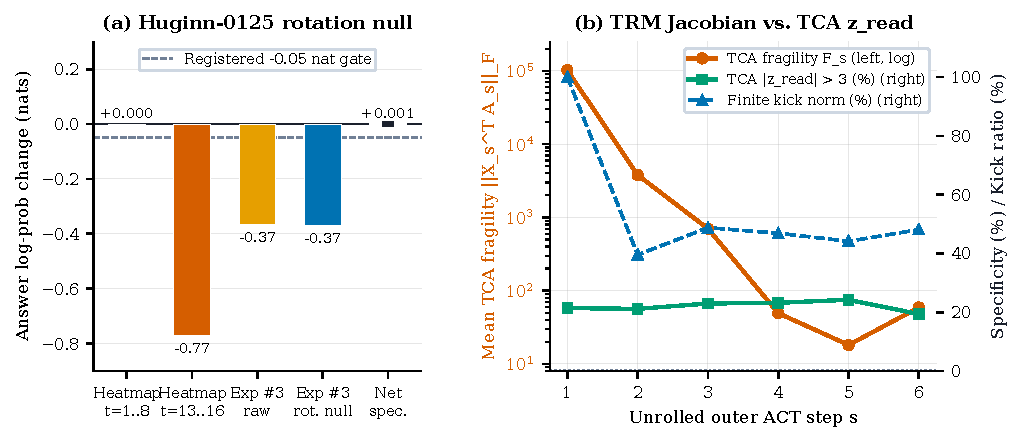
\includegraphics[width=\linewidth]{figures/fig2_fragility_vs_specificity_tca.pdf}
\caption{\textbf{Separating dynamical fragility from directional specificity across BPTT and detached ACT.} \textbf{(a)} Registered \texttt{HUG-CAL-02} (\texttt{Huginn-0125}, $r=16$): large late-window SVD ablation damage ($-0.366$ nats) is matched within $\pm 0.0065$ nats by activation-distribution-matched orthogonal input rotations ($-0.368$ nats), refuting weight-factor specialization. \textbf{(b)} \texttt{LOOPSCOPE-02} \texttt{TRM} unrolled 6-step \texttt{TCA}: 1-step detached ACT induces a $1{,}808\times$ step-1 vs.\ step-6 tangent Jacobian swing ($F_1/F_6$) even while finite $0.25\cdot\mathrm{RMS}$ kicks contract to $30.3\%$; \texttt{TCA}'s closed-form rotation $z$-score cancels $\|A_s\|$ identically, revealing a flat $22.04\%$ read-specific circuit ($81.6\times$ above the $0.27\%$ $3\sigma$ null).}
\label{fig:fragility}
\end{figure}

\subsection{Transported Component Attribution (\texttt{TCA}) and the Lyapunov Dichotomy}

Running multiple forward passes per factor, layer, and iteration window to construct empirical rotation nulls is prohibitively expensive at scale. In \texttt{LOOPSCOPE-01}, we introduced \textbf{Transported Component Attribution (\texttt{TCA})}, which extracts both dynamical fragility and rotation-controlled specificity across every component, layer, and loop step from \emph{a single forward and backward pass}. Let $X_{l,t} \in \mathbb{R}^{P \times d_{\mathrm{in}}}$ be the input activations to weight matrix $W_l \in \mathbb{R}^{d_{\mathrm{out}} \times d_{\mathrm{in}}}$ at loop call $t$, and let $A_{l,t} = \partial y / \partial (X_{l,t} W_l^\top) \in \mathbb{R}^{P \times d_{\mathrm{out}}}$ be the exact gradient of target readout $y$ backpropagated through all remaining iterations $t+1 \dots T$ (transporting downstream repair directly into $A_{l,t}$). Removing a rank-one term $\sigma u v^\top$ writing $(X_{l,t} v)(\sigma u^\top)$ has exact first-order readout effect
\begin{equation}
  \Delta_{l,t}(u,v) \;=\; - \sigma \, v^\top \bigl(X_{l,t}^\top A_{l,t}\bigr) u,
  \qquad
  F_{l,t} \;\triangleq\; \bigl\| X_{l,t}^\top A_{l,t} \bigr\|_F.
  \label{eq:tca}
\end{equation}
Here $F_{l,t}$ is pure \textbf{dynamical fragility}. Under Haar-uniform orthogonal rotation of the read direction $v \mapsto Rv$ (preserving $\|v\|_2$ and output write direction $u$) or write direction $u \mapsto Q u$, $\mathbb{E}[\Delta] = 0$ and the exact closed-form standard deviations yield directional specificity $z$-scores:
\begin{equation}
  z_{\mathrm{read}}(u,v) \;=\; \frac{\Delta_{l,t}(u,v)}{\sigma \|v\|_2 \, \|X_{l,t}^\top A_{l,t} u\|_2 / \sqrt{d_{\mathrm{in}}}},
  \qquad
  z_{\mathrm{write}}(u,v) \;=\; \frac{\Delta_{l,t}(u,v)}{\sigma \|u\|_2 \, \|A_{l,t}^\top X_{l,t} v\|_2 / \sqrt{d_{\mathrm{out}}}}.
  \label{eq:tca_z}
\end{equation}

On \texttt{Huginn-0125} (\texttt{LOOPSCOPE-01} \texttt{Q1}--\texttt{Q2}), summing first-order $\Delta_{l,t}$ over 480 measured multi-iteration ablation conditions achieved Spearman $\rho = 0.75$ and $93\%$ sign agreement for $|\text{measured}| \ge 0.05$ nats (exceeding the registered $\rho \ge 0.60$, $80\%$ validity gate), while reproducing \texttt{HUG-CAL-02} analytically: late iterations are $2.3\times$ more fragile than early iterations, the highest-damage \texttt{core3} factors average $|z_{\mathrm{read}}| \le 1.8$, and only $8.6\%$ of all $4{,}096$ component--step cells exceed $|z_{\mathrm{read}}| > 3$.

Applying unrolled 6-step float32 \texttt{TCA} (105 sequential 2-layer core calls) to the 7M Sudoku \texttt{TRM} in \texttt{LOOPSCOPE-02} prospectively falsified our pre-registered attractor-attenuation hypothesis \texttt{P4} ($\bar{F}_1/\bar{F}_6 \le 0.25$) in the \emph{exact opposite direction}, uncovering a fundamental \textbf{Detached-ACT vs.\ BPTT Lyapunov Dichotomy} (Figure~\ref{fig:fragility}b, Table~\ref{tab:tca_summary}):
\begin{itemize}
  \item \textbf{End-to-end BPTT loopers} (\texttt{Huginn-0125}, \texttt{Lean-CGRT} \texttt{S-loop}, extrapolating \texttt{LoopedChase}) backpropagate gradients through the full unrolled loop during training, penalizing positive tangent Lyapunov exponents and yielding $F_1 / F_{\mathrm{late}} < 1$ ($0.43$ on \texttt{Huginn}; $0.007$ on \texttt{Lean} log-$p$).
  \item \textbf{1-step detached ACT (\texttt{TRM} \cite{jolicoeur2025trm})} detaches $(z_H, z_L)$ between outer supervision steps during training and detaches the first $2$ of $3$ inner $H$-cycles ($12$ of $18$ layer calls per step) under \texttt{torch.no\_grad()}. Macroscopically, nonlinear \texttt{Post-RMSNorm} projection makes the step map strongly contractive to \emph{finite} kicks ($0.25\cdot\mathrm{RMS}$ perturbations decay monotonically from $1.000$ at $s=1$ to $0.303$ at $s=16$). Infinitesimally, however, unconstrained 105-call tangent Jacobians accumulate a mild $\approx 1.074\times$ per-call expansion ($1.074^{105} \approx 1.8\times 10^3$), producing $\bar{F}_1 / \bar{F}_6 = \mathbf{1{,}808.4}$ ($148{,}723$ at $s=1$ vs.\ $21.1$ at $s=5$ on \texttt{L0.down\_proj}, a $6{,}400\times$ swing).
\end{itemize}

This dichotomy carries an immediate methodological consequence for concurrent step-attribution methods such as \texttt{SDI} \cite{kaissis2026sdi}: raw per-step gradient--activation outer products $X_s^\top A_s$ overestimate step-1 influence by three orders of magnitude on detached-ACT models purely from unpenalized tangent Jacobian products. Because $\|A_s\|$ appears identically in the numerator and denominator of Equation~\eqref{eq:tca_z}, \texttt{TCA}'s rotation null cancels Jacobian inflation exactly, revealing a step-invariant \textbf{$22.04\%$ share of read-specific components} ($|z_{\mathrm{read}}| > 3$, $81.6\times$ above the $0.27\%$ Gaussian null; reaching $37.4\%$ on \texttt{L1.down\_proj} at $s=5$) and $12.37\%$ write-specific components. Unlike \texttt{Huginn-0125}'s diffuse settling dynamics, \texttt{TRM}'s tiny reused weights encode highly specific constraint-routing directions at every outer step.

\begin{table}[t]
\centering
\small
\begin{tabularx}{\linewidth}{@{}llccc>{\raggedright\arraybackslash}X@{}}
\toprule
Model & Training gradient & $F_1 / F_{\mathrm{late}}$ & $|z_{\mathrm{read}}|{>}3$ & Finite kick & Mechanistic regime \\
\midrule
\texttt{Nanbeige4.2-3B} & 2-pass BPTT & $0.42$--$2.00$ & $0.9\%$--$8.4\%$ & $6.90\times$ (\texttt{ARG-02}) & Virtual depth; non-contractive \\
\texttt{Qwen3.5-4B-Base} & Untied 36-layer & --- & $0.2\%$--$19.9\%$ & --- & Specific only at final \texttt{L32} ($19.9\%$) \\
\texttt{Huginn-0125} ($r{=}16$) & Multi-step BPTT & $0.43$ & $8.6\%$ & Contractive & Dynamical fragility; \texttt{HUG-CAL-02} null \\
\texttt{Lean S-loop} ($T{=}32$) & Multi-step BPTT & $0.007$ (log-$p$) & $5\%$--$11\%$ & Contractive & Strong attractor masking ($150\times$) \\
\texttt{LoopedChase} ($17/24$) & 8-step BPTT & $0.08$--$0.36$ & High on slots & Contractive & Stationary cursor ($\mathrm{AUC}(F_1/F_8){=}0.950$) \\
\texttt{TRM-7M} (Sudoku) & 1-step detached ACT & $\mathbf{1{,}808.4}$ & $\mathbf{22.04\%}$ & $\mathbf{0.303\times}$ & Basin-contractive, tangent-expansive \\
\bottomrule
\end{tabularx}
\caption{Comparison of \texttt{TCA} fragility ratios $F_1/F_{\mathrm{late}}$, closed-form read specificity shares ($|z_{\mathrm{read}}|>3$; two-sided Gaussian null $= 0.27\%$), and macroscopic perturbation ratios across architectures.}
\label{tab:tca_summary}
\end{table}

\section{Regime II: Closed-Loop Dictionaries, Mediated Variables, and Head-Readable Staircases}\label{sec:regime2}

When a weight-tied model genuinely learns an iterative algorithm via BPTT, can a single sparse basis survive closed-loop re-injection, mediate named algorithmic variables, and expose intermediate states to the model's own readout head without sacrificing depth extrapolation? Controlled experiments in \texttt{RMP} (\emph{Shared Weights, Different Roles II} \cite{dugan2026rmp}) and \texttt{LOOPSCOPE-01} (\texttt{Q3}--\texttt{Q9}, \texttt{Q11}, \texttt{SEM-ECHO-01}) establish \textbf{Regime II}.

\subsection{Closed-Loop Dictionaries and Causal Feature Transfer (\texttt{RMP})}

To eliminate pretraining confounds, \cite{dugan2026rmp} trained matched hidden-dimension-128 transformers across four reference-trace task families (pointer chasing, gated pointer chasing, reachability, and $4\times 4$ Sudoku, depths 1--8): \LoopT\ (one block invoked 8 times, 0.46M parameters) versus \FFU\ (eight untied blocks, 1.84M parameters). All $6/6$ tied seeds passed the $G_0 = 0.98$ exact-match (\texttt{EM}) training gate, compared with $3/6$ untied seeds. Four findings govern sparse surrogates and causal variables in tied loops:
\begin{enumerate}[topsep=3pt,itemsep=2pt]
  \item \textbf{Closed-loop state dictionaries compound gracefully only under shared geometry:} Reconstructing the residual stream through a single shared TopK \texttt{SAE} \cite{gao2024scaling} after \emph{every one of the 8 visits} retained $0.923$, $0.910$, and $0.900$ of clean deep \texttt{EM} (depths 5--8) across \LoopT\ seeds 1--3, satisfying the registered existential \texttt{faithful\_state} rule in all three seeds (strictly beating calibration-error-matched PCA in seeds 2 and 3, and practically tying PCA in seed 1 via widths $2{,}048$/$4{,}096$, $k=32$ by $+12$ and $+11$ of $6{,}000$ examples). Imposing one shared dictionary across the eight blocks of untied \FFU\ seed 3 dropped retention to $0.688$—below both matched PCA ($0.796$) and \emph{equal-norm isotropic Gaussian noise} ($0.778$), proving that coherent basis-mismatch errors compound more destructively across recurrent steps than unstructured noise of identical norm.
  \item \textbf{Live attention rescues shared operation surrogates:} Position-local whole-block transcoders collapsed in closed loop ($\approx 0.17$ relative \texttt{EM}), consistent with cross-position attention carrying $30\%$--$42\%$ of per-step update variance. Replacing only the shared MLP with a single width-4,096 Top-32 transcoder \cite{dunefsky2024transcoders} while keeping native attention live preserved $0.940$--$0.996$ of clean deep \texttt{EM} across 9 models ($4$ original + $5$ fresh seeds) at a $3.5\times$ lower active latent coding rate per position-visit than untied per-layer transcoders ($342$ vs.\ $1{,}213$ bits).
  \item \textbf{Sparse update mediation:} Under donor-update corruption at the answer token, restoring at most 16 shared-dictionary features achieved directional effect fraction $\DEF \ge 0.90$ while beating five subspace baselines (random features, PCA, MLP neurons, random and orthogonal directions) in $63\%$, $91\%$, and $78\%$ of effect-bearing transition classes in \LoopT\ seeds 1--3, requiring a median of $4$--$8$ features.
  \item \textbf{Decodability $\neq$ causal site, and feature-mediated variable transfer:} Linear probes at the answer token decoded early pointer-chase nodes $\cur(s)=f^s(a)$ at $0.76$--$1.00$ accuracy while answer-position interchange patches \cite{geiger2024das,makelov2024illusion} failed ($\IIA \le 0.22$). Patching the \emph{query+answer block} transferred early hops in $5/6$ tied seeds ($\IIA = 0.67$--$1.00$; collision-free start-copy rate $\le 4.5\%$, whereas untied \FFU\ seed 4's apparent $0.50$ \IIA\ was $49.5\%$ start-node copying). In a registered follow-up on $1{,}000$ collision-free counterfactual pairs, $\le 32$ shared-dictionary features transferred $\cur(s)$ ($\IIA \ge 0.60$, beating matched PCA and random subspaces) in $4/5$ eligible tied seeds ($0.605$--$1.000$) and $0/2$ untied seeds ($0.277, 0.386$).
\end{enumerate}

\subsection{Zero Monitorability Trade-Off and Compactification Laws (\texttt{LOOPSCOPE-01})}

In \texttt{LOOPSCOPE-01}, we tested whether forcing intermediate states to remain readable through the model's \emph{own output head} degrades out-of-distribution loop scaling, and derived zero-held-out-label diagnostics predicting when loop extrapolation succeeds (Figure~\ref{fig:compactification}a).

\paragraph{Theorem-proving test-time scaling (\texttt{Q3}, \texttt{Q6}).} On \texttt{Lean-CGRT} mirror proof states, a single-clock tied transformer (\texttt{S-loop}) scaled certified proof success from $48.6\%$ at training budget $T=8$ to $65.0\%$ at test-time budget $T=32$. Applying the model's unmodified output head at intermediate iterations decoded its final chosen tactic on $60\%$ of states at $t=1$ and $94\%$--$99\%$ by $T/2$, accompanied by $150\times$ early log-$p$ fragility attenuation ($F_1/F_{32} = 0.007$) and flat $5\%$--$11\%$ read specificity.

\paragraph{The monitorability frontier on pointer chains (\texttt{Q4}--\texttt{Q9}).} Across 24 depth-8-trained 1.6M-parameter \texttt{LoopedChase} models ($12$ discovery in \texttt{Q4}, $12$ prospective in \texttt{Q5}) spanning intermediate per-loop cross-entropy supervision $\lambda \in \{0, 0.01, 0.1, 1\}$ and architectural variants, \textbf{no monitorability--capability trade-off occurred}: every arm with $\lambda \ge 0.1$ achieved $1.00$ accuracy on held-out depths $9$--$16$ (running $k$ loops at unseen depth $k$) alongside $1.00$ own-head and linear-probe hop readability. Across all 24 arms, 17 extrapolated to depths $9$--$16$ and 7 failed despite $\ge 0.98$ depth-8 training accuracy. Mechanistic dissection across \texttt{Q7}--\texttt{Q9} revealed:
\begin{itemize}
  \item Every arm contracted inside its top-16 cursor PCA subspace ($\kappa_{\mathrm{late}} \in [0.06, 0.74]$) even while full ambient Jacobians expanded ($1.5\times$--$6.9\times$).
  \item The 7 extrapolation failures split cleanly into \emph{deadline schedule desynchronization} ($5/7$ arms, mostly $\lambda=0$, which park or rush updates to meet a memorized loop-8 readout clock) versus \emph{post-depth-8 contraction loss} ($2/7$ arms).
  \item The label-free training-depth fragility ratio $F_1/F_8$ separated extrapolators from failures with $\mathrm{AUC} = 0.950$ ($9/12$ prospective threshold classifications in \texttt{Q5} with zero false alarms; Spearman $\rho = -0.72$), because $F_1/F_8$ tracks \emph{loop non-stationarity}: it correlates $\rho = +0.914$ with cross-step state memory $M$ and aligns with linear decodability $C$ of loop index $t$, which alone achieves $\mathrm{AUC} = 0.958$ (\texttt{Q9}).
\end{itemize}

\begin{figure}[t]
\centering
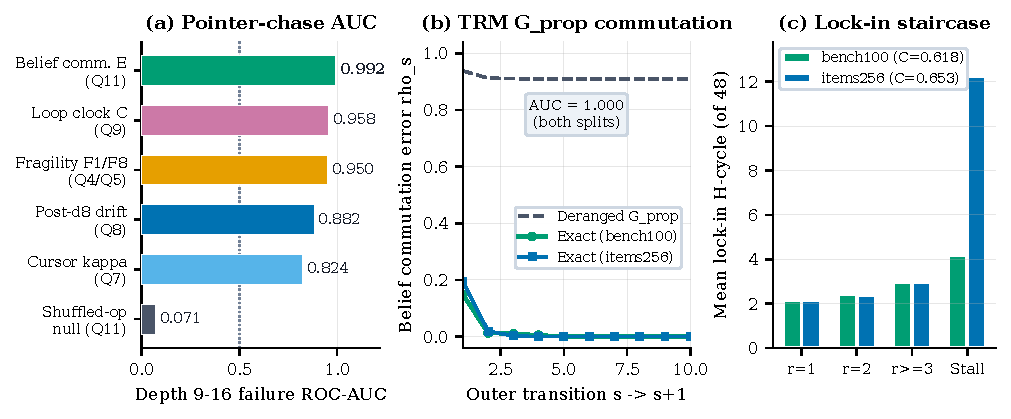
\includegraphics[width=\linewidth]{figures/fig3_compactification_staircase.pdf}
\caption{\textbf{Compactification commutation laws across Markovian pointer chasing (\texttt{LOOPSCOPE-01}) and Sudoku propagation (\texttt{LOOPSCOPE-02}).} \textbf{(a)} ROC-AUC of training-depth diagnostics predicting held-out depth-9--16 failure across 24 \texttt{LoopedChase} models: own-head belief commutation error $\hat{E}$ (\texttt{Q11}) reaches $\mathrm{AUC}=0.992$ (shuffled-operator null $0.071$). \textbf{(b)} On $9\times 9$ Sudoku, \texttt{TRM}'s visible step-$s$ cell marginals commute with exact synchronous propagation $\Gprop$ ($\rho_{\mathrm{clean}} \to 0.000$ by $s=4$) vs.\ deranged board clues ($\rho_{\mathrm{shuf}} \approx 0.91$, $\mathrm{AUC}=1.000$ on both \texttt{bench100} and \texttt{items256}). \textbf{(c)} Across all 48 inner $H$-cycles, cell lock-in times follow the exact deductive staircase $r=1 < r=2 < r\ge 3 < \text{stalled}$ (within-board concordance $C_{\mathrm{stair}} = 0.653$ vs.\ $0.495$ permutation null on \texttt{items256}).}
\label{fig:compactification}
\end{figure}

\paragraph{Compactification-Theory B1 (\texttt{Q11}) and \texttt{Semantic Echo}.} Why do stationary loopers extrapolate? If readout projection $\pi(h_t)$ maps hidden state $h_t$ onto task belief distribution $z_t$ on which one ground-truth step acts via transition operator $G_a$, exact iterative simulation requires the commutation error $\rho_t = \|z_{t+1} - G_a z_t\|$ to vanish across training steps. Evaluating own-head belief commutation error $\hat{E}$ over training loops $4$--$7$ across all 24 \texttt{LoopedChase} models (\texttt{Q11}) achieved \textbf{$\mathrm{AUC}(\hat{E}) = 0.992$} (vs.\ $0.071$ under a shuffled-edge operator null), with $17/17$ extrapolating arms satisfying the finite-horizon simulation bound and a phase-obstruction statistic $\Phi$ isolating all $5/5$ deadline-desynchronized arms. Independently, \texttt{SEM-ECHO-01} showed that trajectory continuation disagreement flags $7/7$ non-extrapolating arms ($\rho = 0.92$).

\section{Regime III: Stationary Attractor Search and the 501-Dimensional Dark Fiber}\label{sec:regime3}

Markovian pointer chains and single-tactic proof steps require no backtracking: the current node $\cur(s)$ is a sufficient statistic for step $s+1$. What happens when a tiny weight-tied transformer solves an NP-complete constraint-satisfaction problem where local deduction stalls and tentative commitments must be revised? In \texttt{LOOPSCOPE-02}, we evaluated a frozen 7M-parameter, 2-layer Attention-\texttt{TRM} (\path{gaoxin492/TinyRecursiveModels-Sudoku-Extreme-att}, \texttt{step\_21700}, hidden size $d=512$, 8 heads, SwiGLU, Post-RMSNorm, 16 outer ACT steps $\times$ 3 $H$-cycles $\times$ 6 $L$-cycles $= 336$ layer passes; replicated on independent checkpoint \path{yagizdevre/trm-sudoku-extreme-att}) on both \texttt{items256} ($256$ stratified boards: $73$ $\Gprop$-solvable, $183$ eventually stalling) and canonical \texttt{bench100} ($100$ boards: $49$ $\Gprop$-solvable, $51$ stalling).

\subsection{Two-Timescale Convergence and Perturbation Repair (\texttt{P1}--\texttt{P3})}

On single target cells (\texttt{items256}, Table~\ref{tab:sudoku_triangulation}), the 7M \texttt{TRM} ($430\times$--$570\times$ smaller than the 3B--4B LLMs) reaches $0.863$ after outer step $s=1$ ($18$ inner passes) and $\mathbf{0.938}$ at $s=16$ ($+0.074$, McNemar $p=3.1\times 10^{-4}$), exceeding \texttt{Qwen3.5-4B-Base} by $+0.727$ ($p=3.8\times 10^{-52}$) and \texttt{Nanbeige4.2-3B} by $+0.809$ ($p=2.4\times 10^{-58}$). Full-board exact solve climbs from $\mathbf{0.082 \to 0.883}$ ($+0.801$) on \texttt{items256} and from $\mathbf{0.210 \to 1.000}$ ($100/100$ boards) on \texttt{bench100} ($0.150 \to 0.920$ on the replication checkpoint).

As summarized in Table~\ref{tab:verdicts}, pre-registered composite verdicts \texttt{P1} and \texttt{P2} returned \texttt{Not supported} for an illuminating structural reason: our single-cell thresholds ($\text{acc}_{16}-\text{acc}_1 \ge 0.25$ and open-loop drop $\ge 0.30$) treated $s=1$ as a shallow pass, whereas \texttt{TRM} factors Sudoku across \textbf{two distinct recurrent timescales}:
\begin{enumerate}[topsep=3pt,itemsep=2pt]
  \item \textbf{Inner 18-pass deductive sweep ($s=1$):} Within a single outer ACT step, 3 $H$-cycles $\times$ 6 $L$-cycles already solve $100\%$ of \texttt{S1\_naked1} and \texttt{S2\_prop2}, $85.9\%$ of \texttt{S3\_prop3plus}, and $59.4\%$ of \texttt{S4\_stalled} target cells ($86.3\%$ overall), while leaving $91.8\%$ of full boards globally incomplete ($0.082$ exact board solve). Consequently, open-loop extrapolation from $z_H(1)$ retains $s=1$'s $0.863$ single-cell score ($-0.074$, $p=3.1\times 10^{-4}$) and donor-$z_H$ displacement drops single-cell accuracy to $0.828$ ($-0.109$, $p=1.9\times 10^{-6}$).
  \item \textbf{Outer steps $s=2\dots 16$ as global constraint-repair attractor:} Across outer steps, full-board exact solve surges by $+80.1$ percentage points ($0.082 \to 0.883$). When 10 empty board cells of $z_H(1)$ are corrupted with donor board states at $s=1$, full-board exact accuracy drops to $\mathbf{0.000}$ ($0/256$) and \textbf{self-repairs across outer steps $2\dots 16$ to $0.887$ ($227/256$, McNemar $p=9.27\times 10^{-69}$)}; direct target-cell donor corruption repairs from $0.723 \to 0.957$ ($+0.234$, $p=2.73\times 10^{-17}$), and $0.25\cdot\mathrm{RMS}$ Gaussian kicks contract monotonically from $1.000 \to 0.303$—the exact dynamical opposite of \texttt{Nanbeige}'s $6.9\times$ kick amplification.
\end{enumerate}

Top-64 SVD usage geometry (\texttt{P3}, graded \texttt{Weak} solely because \texttt{Nanbeige}'s $\bar{r}=0.355$ lay between $0.30$ and $0.40$) confirms that \texttt{TRM} applies a \textbf{stationary outer operator} across steps $s=2\dots 16$ ($\bar{r}_{\mathrm{outer},z_H} = 0.992$, $\bar{r}_{\mathrm{outer},z_L} = 0.994$) while multiplexing inner scratchpad $z_L$ against board-commit $z_H$ calls within each cycle ($\bar{r}_{\mathrm{role}} = 0.765$, dropping to $0.635$ at \texttt{L1.down\_proj}; Figure~\ref{fig:triangulation}b).

\begin{table}[t]
\centering
\small
\begin{tabularx}{\linewidth}{@{}ll>{\raggedright\arraybackslash}p{0.31\linewidth}>{\raggedright\arraybackslash}X@{}}
\toprule
Hypothesis & Verdict & Registered threshold behavior & Structural finding isolated \\
\midrule
\texttt{P1} Triangulation & Not supported & 3/4 met; single-cell $\Delta_{1\to 16} = +0.074 < 0.25$ & Two-timescale split: $s{=}1$ (18 passes) gets $0.863$ single-cell; $s{=}2..16$ drives full-board exact solve $0.082 \to 0.883$ ($+0.801$) \\
\texttt{P2} Attractor vs.\ VD & Not supported & Repair \& \texttt{NB} drift met; single-cell open drop $0.074 < 0.30$ & 10-cell donor board corruption collapses $s{=}1$ exact solve to $0.000$ and self-repairs to $0.887$ ($p=9.3\times 10^{-69}$); kicks contract $0.303\times$ \\
\texttt{P3} SVD geometry & Weak & \texttt{TRM} $\bar{r}_{\mathrm{outer}}=0.992$, $\bar{r}_{\mathrm{role}}=0.765$; \texttt{NB} $\bar{r}=0.355 \in [0.3, 0.4)$ & \texttt{Nanbeige} multiplexes at \texttt{L12}/\texttt{L22} ($0.085, 0.277$) vs.\ \texttt{TRM} stationary outer operator + inner $z_L/z_H$ split \\
\texttt{P4} Unrolled \texttt{TCA} & Not supported & Specificity $22.04\% \gg 1.35\%$; $F_1/F_6 = 1{,}808.4 \gg 0.25$ & Detached-ACT vs.\ BPTT Lyapunov dichotomy: tangent expansion coexists with $0.303\times$ basin contraction; \texttt{TCA} cancels $6{,}400\times$ \texttt{SDI} bias \\
\texttt{P5} Compactification & \textbf{Supported} & \textbf{5/5 sub-criteria met} ($p \le 2\times 10^{-28}$) & Exact $\Gprop$ commutation ($\mathrm{AUC}=1.000$) before stall + 501-dim \texttt{lm\_head}-nullspace dark fiber ($1.000 \to 0.070$) past stall \\
\bottomrule
\end{tabularx}
\caption{Audit of pre-registered \texttt{LOOPSCOPE-02} verdicts alongside the exact structural mechanisms isolated.}
\label{tab:verdicts}
\end{table}

\subsection{Exact $\Gprop$ Commutation Before Stall and the 501-Dimensional Dark Fiber Past Stall (\texttt{P5})}

Hypothesis \texttt{P5} passed all $5/5$ pre-registered criteria on both \texttt{bench100} and \texttt{items256}, unifying Regime II's head-readable staircases with a new phenomenon once local deduction stalls (Figures~\ref{fig:compactification}b--c and \ref{fig:dark_fiber}):

\paragraph{1. Exact $\Gprop$ belief commutation and 48-cycle deductive staircase.} Let $p_s(b) \in \Delta^{81\times 9}$ denote \texttt{TRM}'s visible \texttt{lm\_head} softmax digit probabilities across the 81 cells of board $b$ after outer step $s$, and let $\Gprop(p_s(b), \mathrm{givens}_b)$ apply one soft synchronous naked- plus hidden-single propagation round. On propagation-solvable boards, commutation error $\rho_s(b) = \mathrm{mean}_{i\in\mathrm{empty}}\|p_{s+1}(b,i) - \Gprop(p_s(b),\mathrm{givens}_b)_i\|_2$ falls from $0.148$ ($s=1$) to $0.013$ ($s=2$) and $\mathbf{0.000}$ by $s=4$ on \texttt{bench100} ($0.193 \to 0.019 \to 0.0025 \to 0.000$ on \texttt{items256}), separating exact board clues from deranged clues ($\rho_{\mathrm{shuf}} \approx 0.908$) with \textbf{$\mathrm{AUC} = 1.000$} and $100\%$ paired wins on both splits (Figure~\ref{fig:compactification}b). Across all 48 fine $H$-cycles, mean cell lock-in times strictly track $\Gprop$ deductive round $r(i)$: $2.14$ ($r=1$) $< 2.35$ ($r=2$) $< 2.97$ ($r\ge 3$) $< 12.22$ (stalled) on \texttt{items256} ($2.14 < 2.41 < 2.96 < 4.18$ on \texttt{bench100}), yielding within-board pair concordance $C_{\mathrm{stair}} = 0.6531$ across $95{,}757$ cell pairs versus $0.4947$ under within-board permutation ($0.6177$ vs.\ $0.4951$ across $63{,}032$ pairs on \texttt{bench100}; Figure~\ref{fig:compactification}c).

\begin{figure}[t]
\centering
\includegraphics[width=\linewidth]{figures/fig4_dark_fiber_ablation.pdf}
\caption{\textbf{Post-stall conflict resolution and the 501-dimensional dark fiber.} \textbf{(a)} On \texttt{bench100}, \texttt{TRM} solves $49/49$ propagation-solvable boards and $51/51$ deductively stalled boards (where $\Gprop$ solves $0\%$), driving violated Sudoku units on stalled boards from $13.9 \to 0.0$ via non-monotone cell flips ($107.8$ mean flips). \textbf{(b)} The Monitorability Regime Boundary: Markovian pointer chains (\texttt{LoopedChase}, $\lambda\ge 0.1$) extrapolate and read out through the output head at $1.00$. On Sudoku, resetting scratchpad $z_L \leftarrow L_{\mathrm{init}}$ each outer step costs only $1.0$--$5.1$ pp, whereas projecting $z_H$ onto the 11-dimensional row space of \texttt{lm\_head} (preserving step-$s$ digit logits identically while erasing the 501-d orthogonal dark fiber) collapses exact solve from $1.000 \to 0.070$ on \texttt{bench100} ($p=2.02\times 10^{-28}$) and $0.883 \to 0.066$ on \texttt{items256} ($p=2.43\times 10^{-63}$).}
\label{fig:dark_fiber}
\end{figure}

\paragraph{2. Post-stall conflict traversal and non-monotone revisions.} Where symbolic $\Gprop$ solves $0\%$ of stalled boards by construction, \texttt{TRM} solves $\mathbf{100\%}$ ($51/51$) on \texttt{bench100} and $\mathbf{83.6\%}$ ($153/183$) on \texttt{items256} (Figure~\ref{fig:dark_fiber}a). On solved stalled boards, $98.0\%$ (\texttt{bench100}) and $99.3\%$ (\texttt{items256}) pass through explicit intermediate Sudoku unit violations (mean violated row/column/box units falling from $13.90$ at $s=1$ to $0.00$ by $s=13$ on \texttt{bench100}, and $19.66 \to 5.61$ overall on \texttt{items256}), and $\mathbf{100\%}$ execute non-monotone empty-cell digit commitment flips across the 48 $H$-cycles (mean $107.8$ flips per solved stalled board on \texttt{bench100} and $128.0$ on \texttt{items256}).

\paragraph{3. Causal localization of the 501-dimensional dark fiber.} How does \texttt{TRM} coordinate multi-cell conflict repair without cycling endlessly between locally plausible assignments? Between outer ACT steps $s$ and $s+1$, \texttt{TRM} carries two $512$-dimensional state tensors per token: scratchpad $z_L$ and board state $z_H$. Because \texttt{TRM}'s vocabulary has size $11$ (\texttt{pad}, empty, digits \texttt{1..9}), \texttt{lm\_head.weight} $\in \mathbb{R}^{11 \times 512}$ spans at most an \textbf{11-dimensional readout subspace} $\mathrm{row}(\texttt{lm\_head}) \subset \mathbb{R}^{512}$ with orthogonal projector $\Phead = V_{11} V_{11}^\top$. Its orthogonal complement $(I - \Phead)\mathbb{R}^{512}$ is a \textbf{501-dimensional dark fiber} that is strictly invisible to token readout at step $s$. Comparing two inter-step surgical interventions across all 16 outer steps isolates where search memory lives (Figure~\ref{fig:dark_fiber}b):
\begin{itemize}
  \item \textbf{\texttt{reset\_zL} ($z_L \leftarrow L_{\mathrm{init}}$ before every outer step $s\ge 2$, preserving full $512$-d $z_H$):} Exact full-board solve drops by only $\mathbf{-1.0}$ percentage point on \texttt{bench100} ($1.000 \to 0.990$, McNemar $p=1.0$) and $\mathbf{-5.1}$ percentage points on \texttt{items256} ($0.883 \to 0.832$, $p=2.44\times 10^{-4}$). Inter-step scratchpad persistence is largely dispensable; $z_L$ is reconstructed fresh within each step's 18 inner passes.
  \item \textbf{\texttt{fiber\_erased} ($z_L \leftarrow L_{\mathrm{init}}$ and $z_H^{\mathrm{board}} \leftarrow z_H^{\mathrm{board}}\Phead + H_{\mathrm{init}}(I-\Phead)$ before every outer step $s\ge 2$):} Step-$s$ digit logits and probabilities across all 81 cells are preserved identically ($< 10^{-5}$ numerical tolerance), yet \textbf{exact full-board solve collapses by $-93.0$ percentage points on \texttt{bench100} ($1.000 \to 0.070$, $95\%$ CI $[-0.98, -0.88]$, McNemar $p = 2.02\times 10^{-28}$) and by $-81.6$ percentage points on \texttt{items256} ($0.883 \to 0.066$, $95\%$ CI $[-0.859, -0.766]$, $p = 2.43\times 10^{-63}$)}.
\end{itemize}

Visible digit marginals in $\Phead z_H$ cannot sustain constraint search alone: the 501-dimensional \texttt{lm\_head}-nullspace fiber of $z_H$ carries the coupled parity, elimination, and conflict-history coordinates that steer outer steps out of stalled basins.

\section{Synthesis: The Monitorability Regime Boundary and Outlook}\label{sec:discussion}

\paragraph{The Monitorability Regime Boundary.} Bringing together the monitorability question posed in Section 9 of our September manuscript \cite{dugan2026vpd}, the Markovian pointer-chase frontier of \texttt{LOOPSCOPE-01}, and the Sudoku dark-fiber ablation of \texttt{LOOPSCOPE-02} resolves an apparent tension in latent-reasoning interpretability \cite{olszowiec2026monitoring,sesodia2026inside}: \emph{must latent recurrent reasoning hide computation from the output head to succeed?} The answer depends on a precise structural property of the task's transition operator:
\begin{enumerate}[topsep=3pt,itemsep=2pt]
  \item \textbf{Markovian propagation regimes}—deterministic pointer chasing (\texttt{LoopedChase}), tactic refinement (\texttt{Lean S-loop}), and pre-stall deductive rounds ($r\ge 1$) of Sudoku—have the property that the current visible belief distribution $z_t \in \Delta$ is a sufficient state for the next transition $z_{t+1} = G z_t$. Here, looped transformers naturally form (or can be supervised via $\lambda \ge 0.1$ to form) \textbf{head-readable compactifications} ($\rho_t \to 0$) with \emph{zero capability penalty}, and training-depth commutation error predicts out-of-distribution depth scaling ($\mathrm{AUC}=0.992$).
  \item \textbf{Non-monotone constraint-search regimes}—such as post-stall NP-complete Sudoku—cannot factor through per-cell readout marginals $\Phead z_H$: two search states with identical single-cell digit probabilities can represent incompatible joint assignments or opposite conflict histories. Resolving coupled unit violations via $100+$ non-monotone cell flips mathematically requires state dimensions orthogonal to the readout head. In \texttt{TRM}, that role is fulfilled by the $501$-dimensional dark fiber $(I-\Phead)z_H$, explaining why intermediate-logit monitoring sees smooth staircases before stall yet misses $93\%$ of the causal state driving post-stall search.
\end{enumerate}

\paragraph{Scope boundaries and methodological limitations.} Four explicit boundaries govern our conclusions. First, the capability gap between \texttt{Nanbeige4.2-3B}/\texttt{Qwen-4B} and the 7M \texttt{TRM} on Sudoku separates in-context 3-shot inference in general-purpose pretrained language models from supervised recursive puzzle training; it shows that 2-pass LM weight tying does \emph{not} spontaneously induce recursive search on combinatorial grids, not that billion-parameter loopers could never be trained via detached ACT to do so. Second, exact float32 unrolled \texttt{TCA} on \texttt{TRM} was bounded at 6 outer steps (105 layer calls) by 16~GB GPU memory; extending memory-checkpointed backpropagation to all 16 steps will test whether tangent Lyapunov growth plateaus near fixed points. Third, in \texttt{Nanbeige4.2-3B} \cite{dugan2026vpd}, Muon \texttt{SAE} change-fidelity mismatch was shown to stem from discrete top-$k$ support switching, leaving open whether continuous gated or JumpReLU dictionaries with Jacobian regularization can track cross-pass perturbations without support spikes. Fourth, dark-fiber necessity is established here on $9\times 9$ Sudoku; testing universality requires a second non-monotone domain.

\paragraph{Prospective \texttt{ARC-AGI-2} dark-fiber protocol.} Because \texttt{TRM} checkpoints trained on \texttt{ARC-AGI-2} \cite{jolicoeur2025trm} use an identical $d=512$ residual stream and an $11$-token grid color head (\texttt{pad} plus colors \texttt{0..9}; $\mathrm{rank}(\Phead) \le 11$, orthogonal fiber dimension $501$) over $30\times 30$ grid tokens, our \texttt{reset\_zL} and \texttt{fiber\_erased} interventions transfer with \emph{zero architectural modification}. Measuring exact-grid solve retention under $\Phead$ projection across \texttt{ARC-AGI-2} tasks stratified by single-step cellular rule vs.\ multi-object hypothesis revision provides an immediate, parameter-free prospective test of the Monitorability Regime Boundary beyond Sudoku.

\bibliographystyle{plain}
\bibliography{references}

\end{document}
